\chapter{Realizace Laser Game systému}

 V této kapitole se budu zabývat jednotlivými částmi Laser Game systému a popisem souvislostí mezi jednotlivými bloky z kterých jsou tyto části vytvořeny.

\section{Vesta}

Vesta je rozdělena do několika bloků, aby byl její návrh jednodušší a také modulárnější, aby v případě potřeby úpravy parametrů stačilo upravit jen požadovaný blok.

\begin{figure}[H]
    \begin{center}
        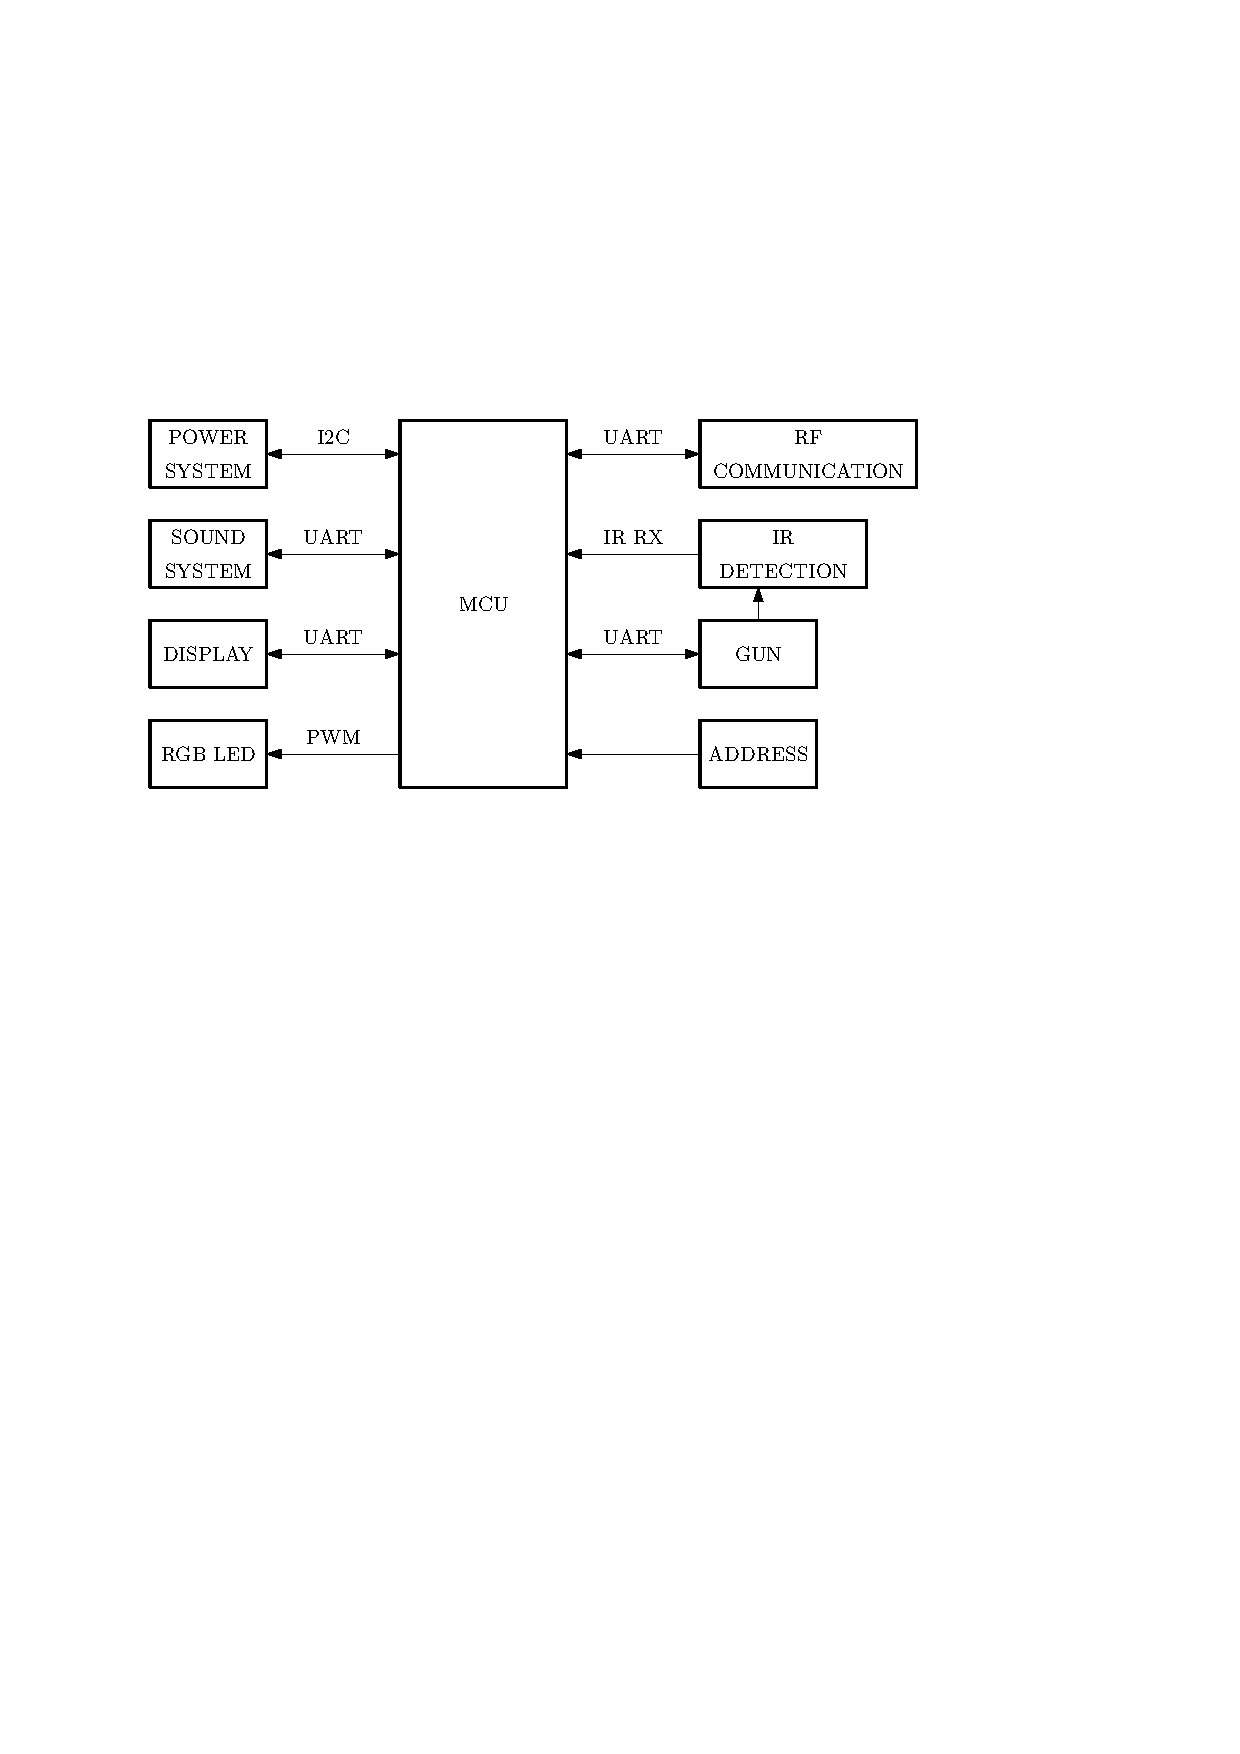
\includegraphics[width=\textwidth]{img/vest-system}
    \end{center}
    \caption{blokové schéma vesty}
\end{figure}

Řídící jednotkou vesty je 32~\jedn{b} MCU STM32F405RGT založený na ARM jádru Cortex M4, jeho základními parametry jsou 1~\jedn{MB} FALSH paměti a 192~\jedn{kB} RAM.

MCU využívá čtyř separátních UART sběrnic pro komunikaci ze subsystémy vesty. Prostřednictvím RF modulu HM-TRP zajišťuje komunikaci z routerem. Zpracovává příchozí data z rádiového modulu a podle nich nastavuje parametry vesty či posílá routeru informace.

Další úlohou řídícího MCU je zpracovávání dat z IR detektoru. Podle nich dochází k vyhodnocování zásahů hráče, pokud k zásahu dojde nebo je hráč z jiného důvodu vyřazen ze hry, pošle řídící MCU příkaz do zbraně aby byla zablokována střelba. Jakmile může hráč opět ve kře pokračovat pošle do zbraně příkaz k odblokování.

Řídící MCU také generuje PWM signál určený k nastavování barvy RGB LED.

Pokud je třeba sdělit hráči nějakou informaci, tak v závislosti na nastavení hry může řídící MCU aktivovat zvukový subsystém, vypsat údaje na displej nebo použít RGB LED.

Po zapnutí si MCU zjistí svou adresu pomocí GPIO portu nastaveného jako vstupní s vnitřním pull-up rezistorem. Adresa je HW podle osazení rezistorů na PCB. Tato adresa je poté využívána v RF i IR komunikaci.

Poslední důležitou úlohou MCU je komunikace s napájecím subsystémem a monitorování stavu akumulátoru.


\section{Zbraň}
\begin{figure}[H]
    \begin{center}
        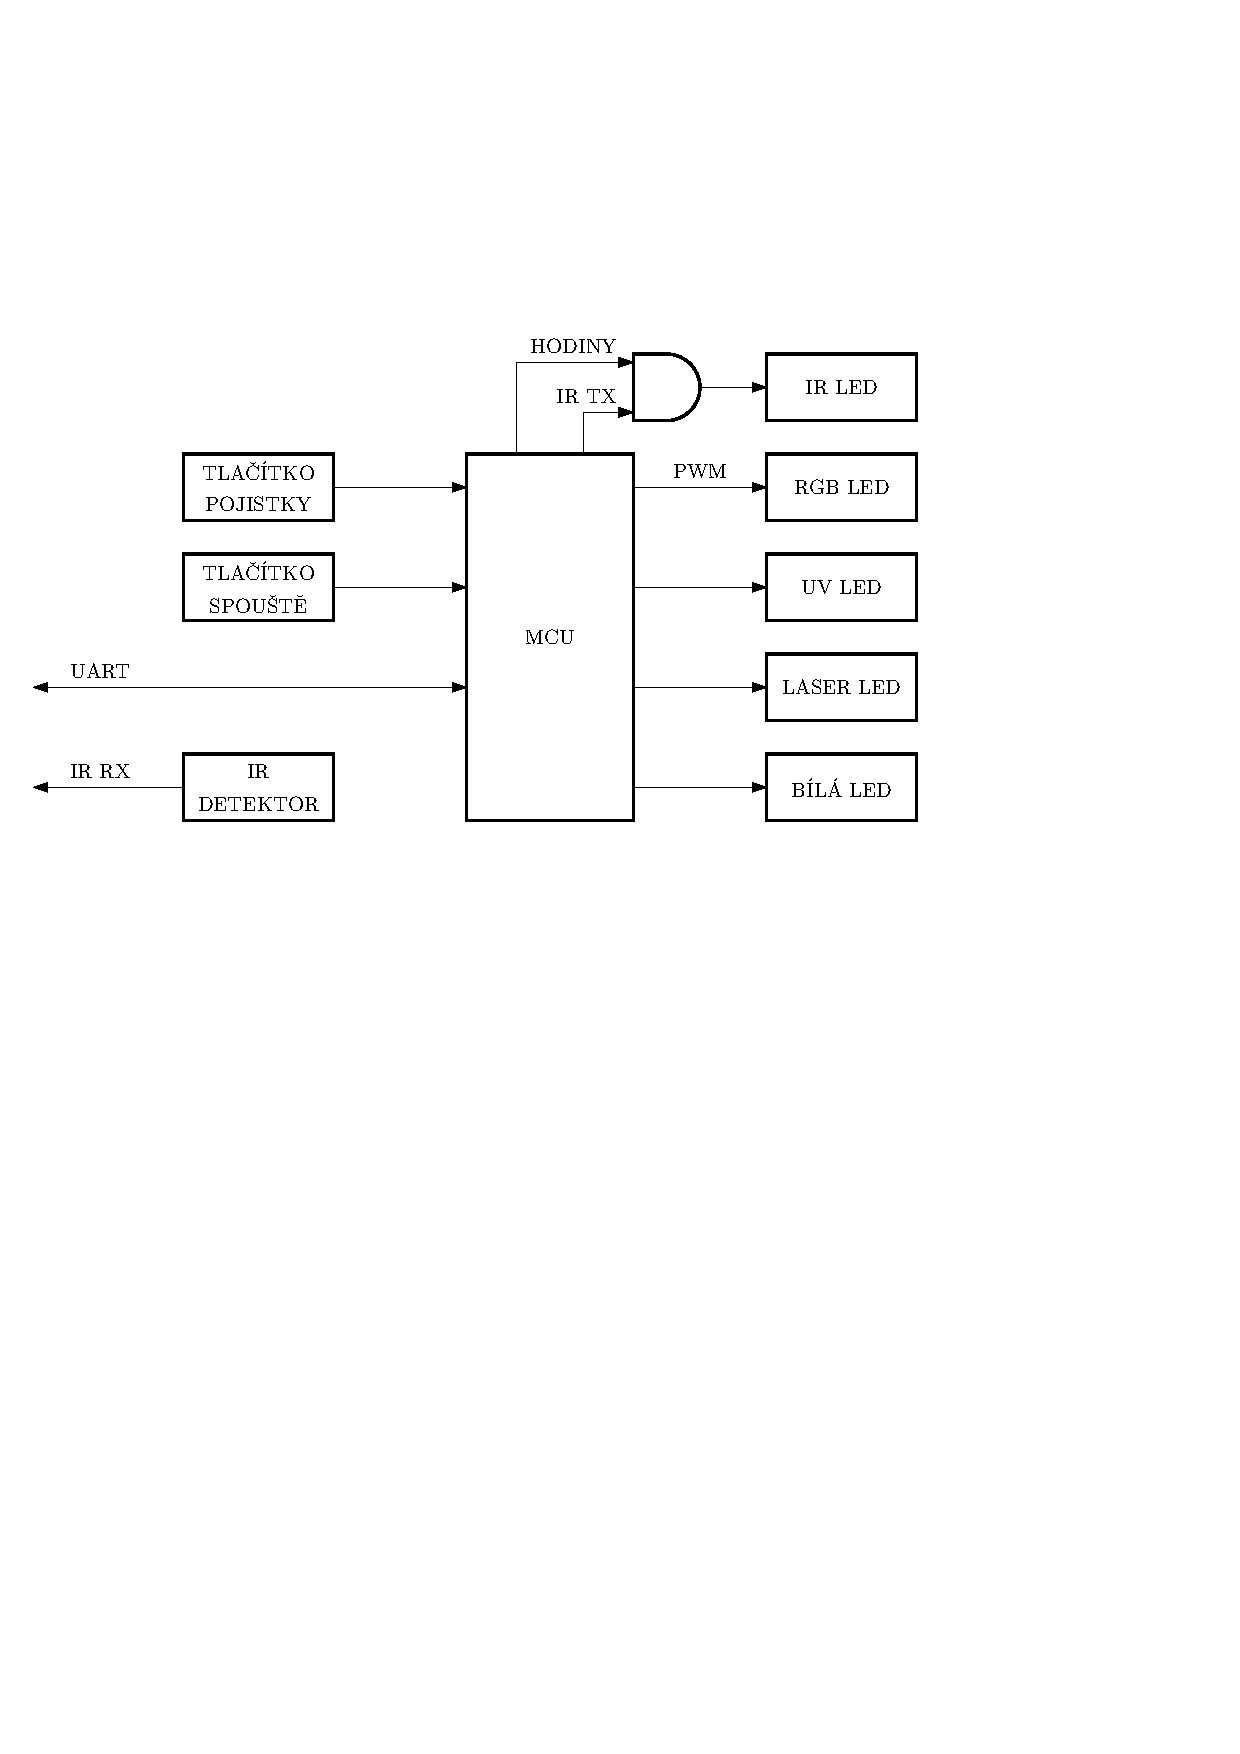
\includegraphics[width=\textwidth]{img/gun}
    \end{center}
    \caption{blokové schéma zbraně}
\end{figure}
Hlavním funkcí zbraně je vysílání RF signálu. Ten je generován MCU STM32F042F6P, který je založený na ARM jádru Cortex M0. Je vybaven 32~\jedn{kB} FLASH a 6~\jedn{kB} SRAM. Generovaný IR signál je složen ze dvou signálů a to nosného a datového. tyto dva signály jsou směšovány dohromady pomocí hradla AND a následně je jím ovládána vysílací IR LED.

Zbraň dále obsahuje laserovou diodu, využívanou ke znázornění místa, kam hráč střílí. Dále jsou ve zbrani dostupné bílá, UV a RGB LED, které svítí v závislosti na nastavení hry.

Zbraň je vybavena dvěma tlačítky, spouští, která slouží k ovládání vysílání a pojistkou jejíž funkce závisí na nastavení hry. Buď je jejím stiskem podmíněna střelba a nebo je používána k ovládání svítilny realizované bílou či UV LED.

Ve zbrani je také vybavena IR detektorem, který není nijak spojen s MCU zbraně, nýbrž je propojen přímo z detekčním systémem vesty.

Komunikace mezi řídícím MCU vesty a MCU zbraně probíhá prostřednictvím UART sběrnice. Ze zbraně po této sběrnici přichází povolení a zákazy střelby, případně nastavení RGB LED, naopak zbraň se ptá vesty na její adresu a nastavení RGB.

\section{Router}
\begin{figure}[H]
    \begin{center}
        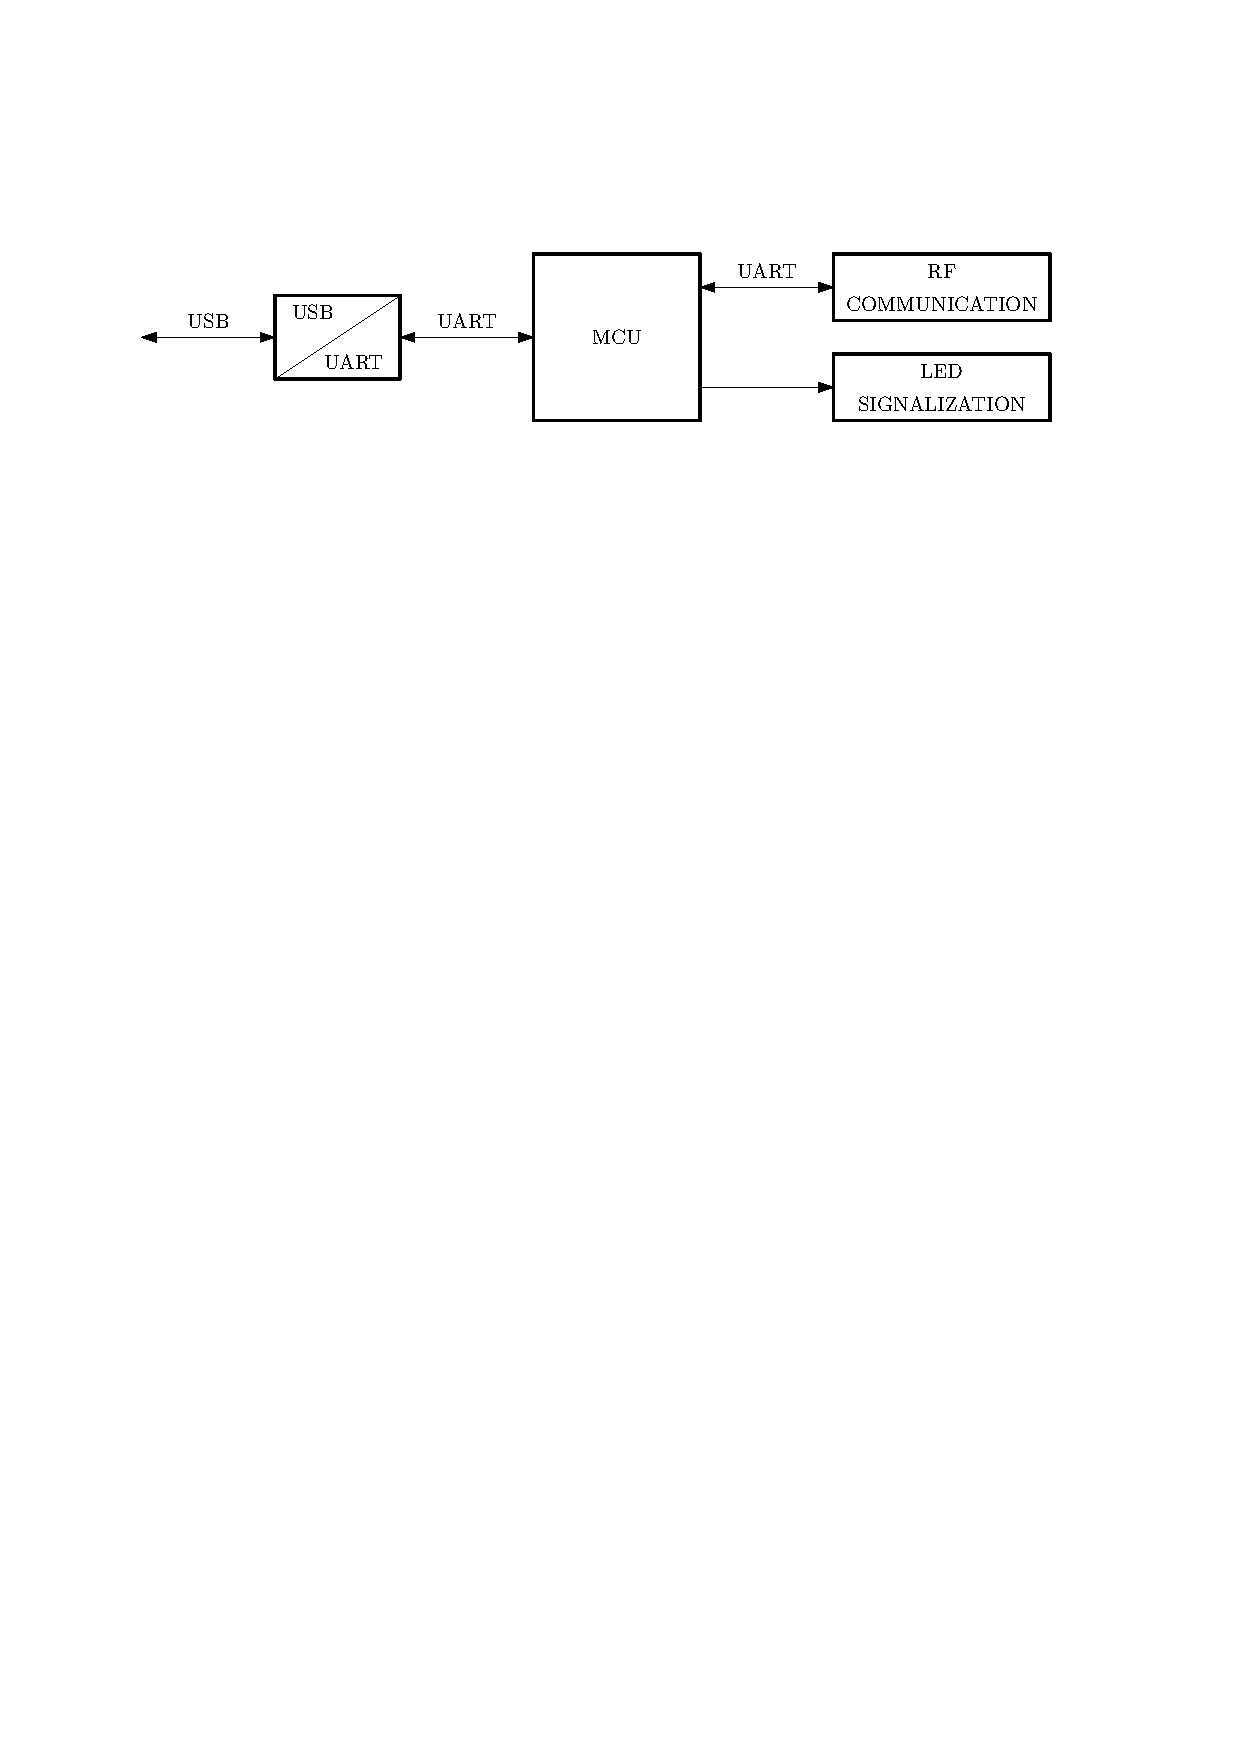
\includegraphics[width=\textwidth]{img/router}
    \end{center}
    \caption{blokové schéma routeru}
\end{figure}
Pomocí RF modulu zajišťuje komunikaci ze zařízeními v síti. Je také vybaven MCU STM32F405RGT, které je pro co nejrychlejší zpracovávání rámců z vest taktováno na 160~\jedn{MHz}. Na základě požadavků z řídícího počítače nastavuje zařízení v síti. Přiděluje zařízením v síti komunikační okna a získané informace ze zařízení zasílá opět do řídícího počítače. Zajišťuje také jednotné časování vest v síti.
